\begin{frame}[fragile]{Visualização da decomposição do sinal}

    \begin{figure}
        \centering

        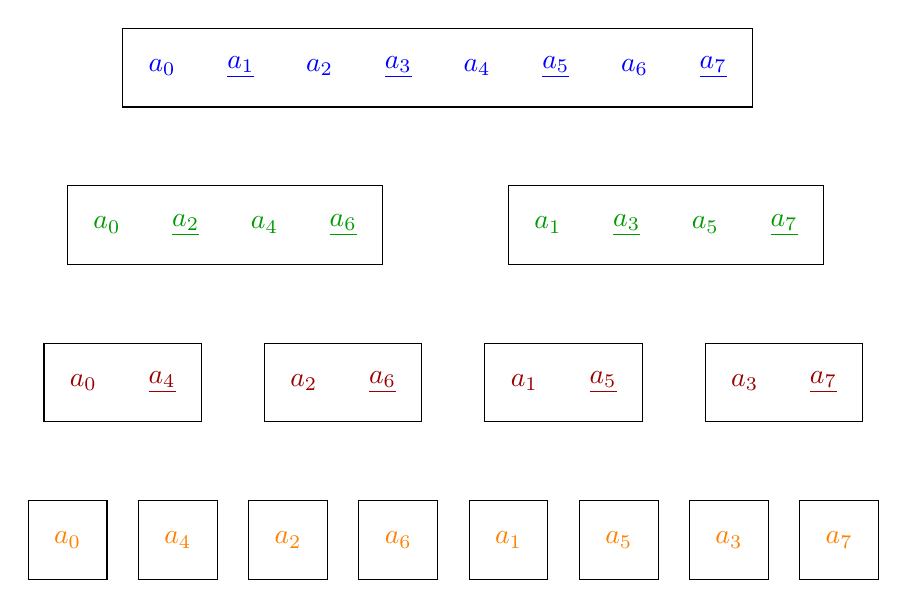
\begin{tikzpicture}

           \draw (1.2, 6) rectangle (9.2, 7);

           \foreach \x in {1,...,4}
           {
                \pgfmathtruncatemacro{\label}{2*\x - 2};
                \node at (2*\x - 1 + 0.7, 6.5) { \textcolor{blue}{{$a_{\label}$}} };
           }

           \foreach \x in {1,...,4}
           {
                \pgfmathtruncatemacro{\label}{2*\x - 1};
                \node at (2*\x + 0.7, 6.5) { \textcolor{blue}{\underline{$a_{\label}$}} };
           }

           \foreach \x in {0,...,1}
                \draw (4*\x + 0.4*4*\x + 0.5, 4) rectangle (4*\x + 0.4*4*\x + 4.5, 5);

           \foreach \x in {0,...,1}
           {
                \pgfmathtruncatemacro{\label}{4*\x};
                \node at (2*\x + 1, 4.5) { \textcolor{green!60!black}{{$a_{\label}$}} };
           }

           \foreach \x in {0,...,1}
           {
                \pgfmathtruncatemacro{\label}{4*\x + 2};
                \node at (2*\x + 2, 4.5) { \textcolor{green!60!black}{\underline{$a_{\label}$}} };
           }

           \foreach \x in {0,...,1}
           {
                \pgfmathtruncatemacro{\label}{4*\x + 1};
                \node at (2*\x + 6.6, 4.5) { \textcolor{green!60!black}{{$a_{\label}$}} };
           }

           \foreach \x in {0,...,1}
           {
                \pgfmathtruncatemacro{\label}{4*\x + 3};
                \node at (2*\x + 7.6, 4.5) { \textcolor{green!60!black}{\underline{$a_{\label}$}} };
           }

           \node at (0.7, 2.5) { \textcolor{red!60!black}{$a_0$} };
           \node at (1.7, 2.5) { \textcolor{red!60!black}{\underline{$a_4$}} };
 
           \node at (3.5, 2.5) { \textcolor{red!60!black}{$a_2$} };
           \node at (4.5, 2.5) { \textcolor{red!60!black}{\underline{$a_6$}} };

           \node at (6.3, 2.5) { \textcolor{red!60!black}{$a_1$} };
           \node at (7.3, 2.5) { \textcolor{red!60!black}{\underline{$a_5$}} };

           \node at (9.1, 2.5) { \textcolor{red!60!black}{$a_3$} };
           \node at (10.1, 2.5) { \textcolor{red!60!black}{\underline{$a_7$}} };

           \foreach \x in {0,...,3}
                \draw (2*\x + 0.4*2*\x + 0.2, 2) rectangle (2*\x + 0.4*2*\x + 2.2, 3);

            \foreach \x in {0,...,7}
                \draw (\x + 0.4*\x, 0) rectangle (\x + 0.4*\x + 1, 1);

           \node at (0.5, 0.5) { \textcolor{orange}{$a_0$} };
           \node at (1.9, 0.5) { \textcolor{orange}{$a_4$} };
           \node at (3.3, 0.5) { \textcolor{orange}{$a_2$} };
           \node at (4.7, 0.5) { \textcolor{orange}{$a_6$} };
           \node at (6.1, 0.5) { \textcolor{orange}{$a_1$} };
           \node at (7.5, 0.5) { \textcolor{orange}{$a_5$} };
           \node at (8.9, 0.5) { \textcolor{orange}{$a_3$} };
           \node at (10.3, 0.5) { \textcolor{orange}{$a_7$} };

        \end{tikzpicture}

    \end{figure}

\end{frame}
